\chapter{Resultados Experimentais Preliminares}
\label{cap:resultados}

Este capítulo apresenta os resultados experimentais preliminares obtidos por este trabalho até o momento da escrita deste documento. Inicialmente, ele descreve a infraestrutura experimental utilizada. Em seguida, analisa as três tarefas de Physical Design. Por fim, apresenta uma síntese dos resultados e apresenta algumas melhorias e expectativas dos trabalhos a serem realizados até o a conclusão do mestrado.

\section{Infraestrutura experimental}
\label{sec:infraestrutura_experimental}

Os experimentos realizados utilizaram o conjunto de benchmarks disponibilizados pela competição \textit{ICCAD 2015 CAD Contest (problem C: Incremental Timing-Driven Placement)} \cite{kim2015}, o qual inclui 8 circuitos que possuem entre 768k e 1,93M células, todos derivados de circuitos industriais. Optou-se por utilizar tal infraestrutura pois a mesma disponibiliza circuitos com número de células compatível com circuitos contemporâneos. Além disso, tal infraestrutura é de acesso aberto, o que facilita a comparação experimental deste trabalho com futuros trabalhos que possivelmente serão realizados por terceiros. Como biblioteca básica, utilizou-se a Ophidian: Open-Source Library for Physical Design Research and Teaching~\cite{ophidian}.

Todos os experimentos foram executados em um computador Linux com processador Intel\textsuperscript{\textregistered} Core\textsuperscript{\textregistered} i5-4460 CPU @ 3.20~GHz.
A Figura~\ref{fig:architectureMemoryZeus} apresenta de forma gráfica a arquitetura deste computador.
Este computador possui 32GB~RAM (DDR3 a 1600MHz) como memória principal.
Seu processador possui quatro núcleos idênticos e três níveis de cache.
Os primeiros dois níveis de cache~(L1 and L2) são privados para cada core do processador e possuem 64KB e 256KB de capacidade respectivamente.
O terceiro nível da cache~(L3) é compartilhado entre todo o processador e possui 6144KB de capacidade.

\begin{figure}[ht]
    \centering
    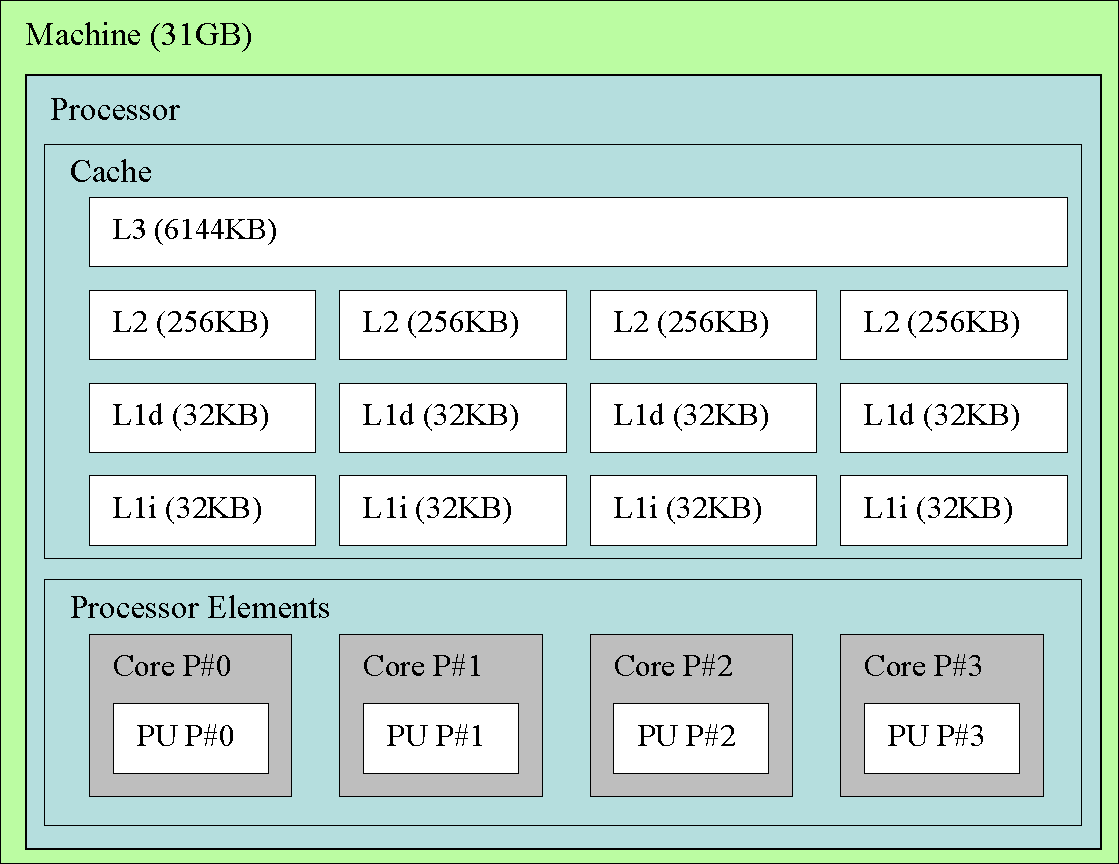
\includegraphics[width=0.5\linewidth]{img/results/architectureMemoryZeus.pdf}
    \caption{Arquitetura do computador utilizados nos experimentos.}
    \label{fig:architectureMemoryZeus}
\end{figure}

Os experimentos que avaliam o tempo de execução podem apresentar resultados diferentes em cada realização, devido a variações causadas pelo computador utilizado. Portanto, para aumentar a confiança estatística obtida pelos experimentos, os mesmos foram repetidos 30 vezes.% , o que resultou em 99\% de confiança estatística\footnote{A confiança estatística foi medida utilizando o teste t de Student para p=0,01.}.

\section{Metodologia Experimental}
\label{sec:metodologia_experimental}

Para avaliar o impacto que a organização dos dados pode causar em problemas de \textit{Physical Design}, será avaliado o \textbf{número de cache misses} e o \textbf{tempo de execução} para três problemas. São eles:
\begin{itemize}
    \item Problema A: Verificar se cada célula do circuito está contida dentro dos  limites físicos do chip. Neste cenário somente uma propriedade é necessário para cada célula. Portanto, a localidade dos dados será totalmente explorada na implementação com \ac{dod}. Sendo assim, este problema representa o melhor caso para implementações com o modelo de dados \ac{dod}.
    \item Problema B: Estimar o comprimento de todas as interconexões do circuito. Este cenário acessa diferentes propriedades das entidades. Portanto, não pode explorar eficientemente a localidade de dados fornecida por \ac {dod}, uma vez que as propriedades dos pinos em uma única interconexão podem não ser contíguas na memória, a menos que a matriz de propriedades esteja previamente ordenada.
    \item Problema C: Clusterização de Registradores. Este cenário representa uma tarefa mais complexa que pertence a síntese física de um \ac{ic}.
\end{itemize}

Para cada problema listado acima, foram implementados protótipos de software seguindo duas organizações de dados: \ac{ood} e \ac{dod}.
Estes protótipos foram implementados utilizando linguagem de alto nível C++ e o código fonte encontra-se disponível online no repositório GitHub da Ophidian~\cite{ophidian}.

As Subseções \ref{sec:problema_a} a \ref{sec:problema_c} a seguir apresentam os resultados preliminares para os três problemas avaliados.
Todos os resultados apresentados nestas seções são a média de 30 execuções. 
Por fim, a Subseção \ref{sec:sintese_resultado} apresenta uma síntese de todos os resultados.

\section{Estudo de Caso A:}
\label{sec:problema_a}

A Figura \ref{fig:missProblemA} apresenta o número de cache misses (eixo Y) em milhões para cada circuito avaliado (eixo X). As barras vermelhas representam o modelo de dados Orientado a Objetos (\ac{ood}). As barras azuis representam o modelo Orientado a Dados (\ac{dod}). O número total de cache misses para o \ac{dod} (de $0.5M$ a $1.4M$) foi, em média, um décimo do número atingido pelo modelo \ac{ood} (de $5.4M$ a $13.7M$). A redução no número de cache misses é proveniente diretamente da melhor organização dos dados em memória. Nesta organização, os dados de uma mesma propriedade (posição de uma determinada célula neste problema) estão armazenados contiguamente em memória. Portanto, ao ocorrer um miss na cache, somente dados úteis são recuperados da memória principal. Assim, é realizado um melhor aproveitamento dos blocos de dados recuperados da memória principal para a cache. 

\begin{figure}[ht]
    \centering
    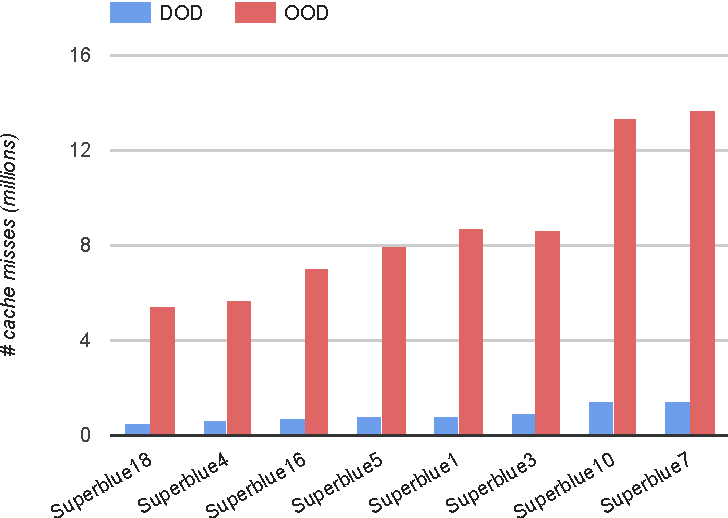
\includegraphics[width=0.7\linewidth]{img/results/missProblemA}
    \caption[Cache misses do Problema~A.]{Número de cache misses resultantes dos dois protótipos de software do Problema~A.}
    \label{fig:missProblemA}
\end{figure}

A exploração da localidade de dados reduz o tempo de acesso à memória principal, que representa o gargalo principal. Esta redução no tempo de acesso a memória pode ser observada na Figura~\ref{fig:runtimeProblemA}. Este gráfico retrata o tempo de execução (eixo Y) em milissegundos para cada circuito avaliado (eixo X). Pode-se observar que a versão \ac{dod} executou mais rápido em todos os circuitos avaliados. Os tempos de execução da versão \ac{dod} foram entre $4ms$ e $12ms$, enquanto os tempos de execução de \ac{ood} foram entre $74ms$ e $186ms$. Portanto, para o problema~A, \ac{dod} é em média $94\%$ ($16\times$) mais rápido do que \ac{ood}.

\begin{figure}[ht]
    \centering
    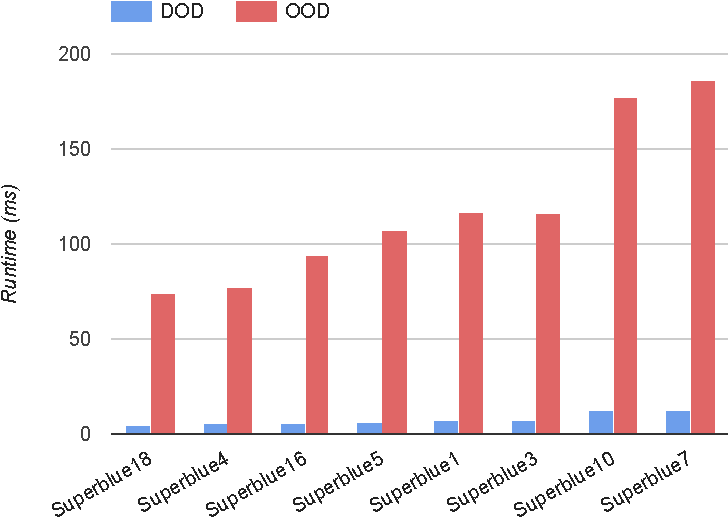
\includegraphics[width=0.7\linewidth]{img/results/runtimeProblemA}
    \caption[Tempo de execução Problema~A]{Tempo de execução para o Problema~A.}
    \label{fig:runtimeProblemA}
\end{figure}

\section{Estudo de Caso B:}
\label{sec:problema_b}

Com objetivo de avaliar o impacto da organização dos dados no pior cenário para o \ac{dod}. Nesta etapa do trabalho foi avaliado uma tarefa que necessite de diversas propriedades para solucionar o problema. 
Diferente do Estudo de Caso~A, nesta tarefa é necessário acessar diferentes \textit{entity-component systems} (interconexões e pinos) e múltiplas propriedades. Complementarmente, os pinos pertencentes a cada interconexão podem não estar contíguos em memória, o que impacta na performance. 

A Figura~\ref{fig:runtimeProblemB} apresenta o número de cache misses resultantes para cada modelo de programação. Pode-se observar que o número de cache misses do \ac{dod} (de $253M$ a $819M$) foi, em média, $10\%$ maior do que quando comparado ao modelo \ac{ood} (de $231M$ a $749M$). O maior número de cache misses do \ac{dod} resultou em uma performance inferior para o Problema~B. Contudo, o modelo \ac{dod} ainda proporcionou uma melhor engenharia de software. Adicionalmente, a diferença de performance no Problema~B (quando o \ac{dod} é mais lento) é muito menor do que a performance atingida no Problema~A (quando o \ac{dod} é mais rápido).
 
\begin{figure}[ht]
    \centering
    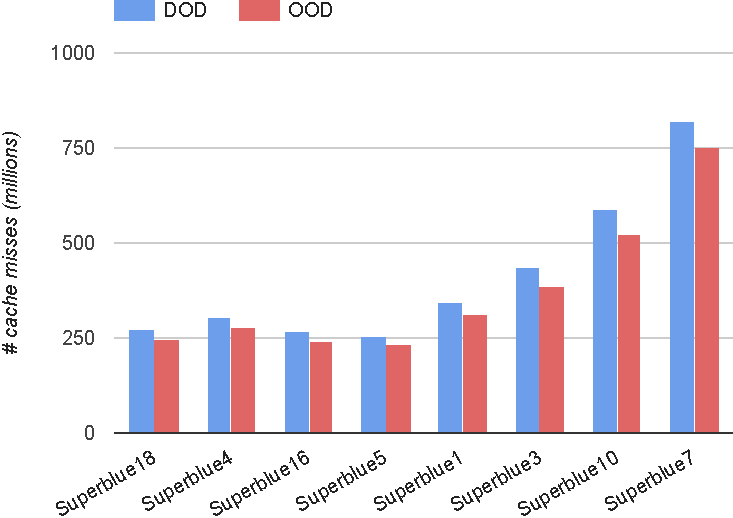
\includegraphics[width=0.7\linewidth]{img/results/missProblemB}
    \caption[Cache misses do Problema~B.]{Número de cache misses resultantes dos dois protótipos de software do Problema~B.}
    \label{fig:missProblemB}
\end{figure}

Na Figura~\ref{fig:runtimeProblemB} esta apresentado o tempo de execução (eixo Y) em milissegundos para cada circuito avaliado (eixo X). O tempo de execução para o \ac{dod} foi entre $3497ms$ e $10300ms$, enquanto o tempo de execução do \ac{ood} foi $3306ms$ e $9654ms$. Como consequência do maior número de cache misses, no Problema~B o modelo \ac{ood} foi em média $6\%$ mais rápido do que o modelo \ac{dod}.

\begin{figure}[ht]
    \centering
    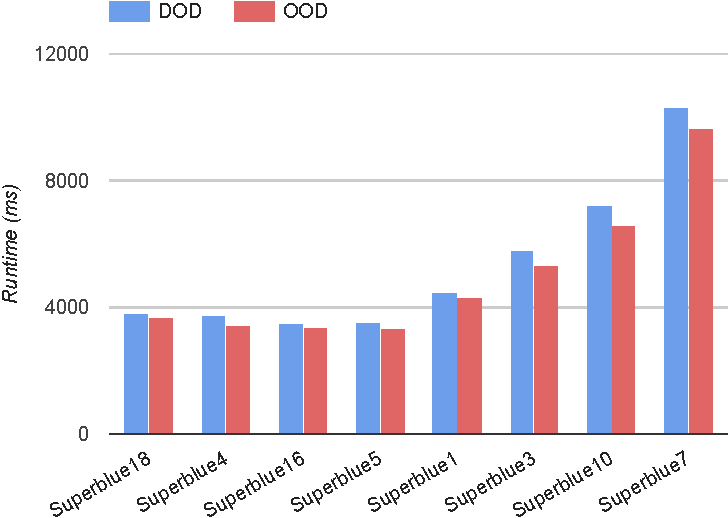
\includegraphics[width=0.7\linewidth]{img/results/runtimeProblemB}
    \caption[Tempo de execução Problema~B]{Tempo de execução para o Problema~B.}
    \label{fig:runtimeProblemB}
\end{figure}

\section{Estudo de Caso C:}
\label{sec:problema_c}

A Clusterização de Registradores consiste em identificar células síncronas próximas e agrupa-las em um único \textit{cluster}. Para resolver este problema foi implementado o algoritmo clássico K-Means~\cite{selim1984k}. K-Means é um algoritmo clássico de agrupamento de elementos, não utilizado somente para register clustering, mas também em diferentes áreas como: \textit{machine learning} e \textit{data mining}.

Para avaliar como a organização dos dados pode impactar no desempenho desta tarefa, foram implementados duas versões (sequencial e paralela) para cada modelo de organização dos dados (\ac{ood} e \ac{dod}).
A Subseção~\ref{subsec:execucaoSequencialProblemaC} irá discutir os resultados preliminares para a execução sequencial, ao passo que, a Subseção~\ref{subsec:execucaoParalelaProblemaC} ira abordar os resultados da execução paralela.

\subsection{Execução Sequencial}
\label{subsec:execucaoSequencialProblemaC}

A Figura~\ref{fig:missProblemC_sequential_rtree} apresenta o número total de cache misses (eixo Y) em milhões para cada circuito avaliado (eixo X).  
O número de cache misses para a Orientação a Dados (\ac{dod}) (de $17M$ a $173M$) foi, em média, $24\%$ menor do que o número requerido pela Orientação a Objetos (\ac{ood}) (de $29M$ a $214M$).
Este resultado indica, como o esperado, que a localidade espacial foi melhor utilizada quando aplicou-se o \ac{dod}.

\begin{figure}[ht]
    \centering
    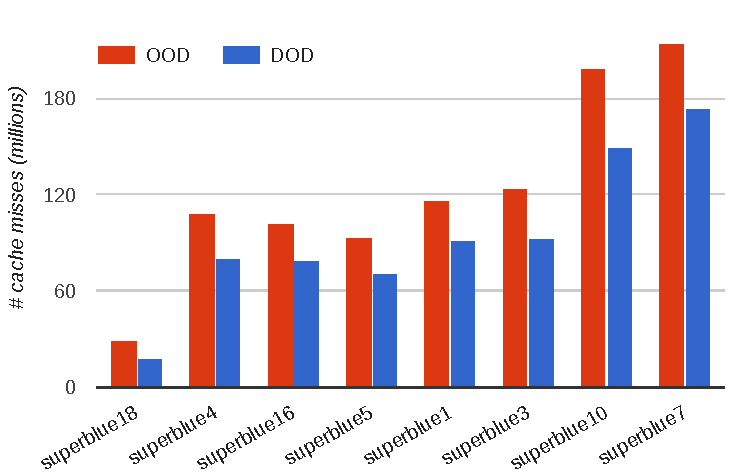
\includegraphics[width=0.7\linewidth]{img/results/missProblemC_sequential_rtree}
    \caption[Cache misses Problema~C versão sequencial]{Número de cache misses para a implementação sequencial da Clusterização de Registradores}
    \label{fig:missProblemC_sequential_rtree}
\end{figure}

O menor número de cache misses com \ac{dod} impactou no tempo de execução para esta tarefa.
A Figura~\ref{fig:runtimeProblemC_sequential_rtree} apresenta a média dos tempos de execuções (eixo Y) em milissegundos para cada circuito avaliado (eixo X).
O tempo necessário para o \ac{dod} concluir a tarefa foi entre $724ms$ e $2364ms$, enquanto quando utilizado o \ac{ood} foi entre $804ms$ e $2526ms$.
Em média, o \ac{dod} executou $7.5\%$ mais rápido que o \ac{ood}.
Portanto, estes resultados confirmam que uma melhor organização dos dados em memória podem impactar beneficamente no tempo de execução de tarefas de \textit{Physical Design}.

Pode-se notar também que a redução no número de cache misses não impactou na mesma proporção no tempo de execução. Isto se deve ao fato de que a organização dos dados impactou somente em instruções de acesso a dados em memória, sendo este conjunto um subconjunto de todas as instruções do software.

\begin{figure}[ht]
    \centering
    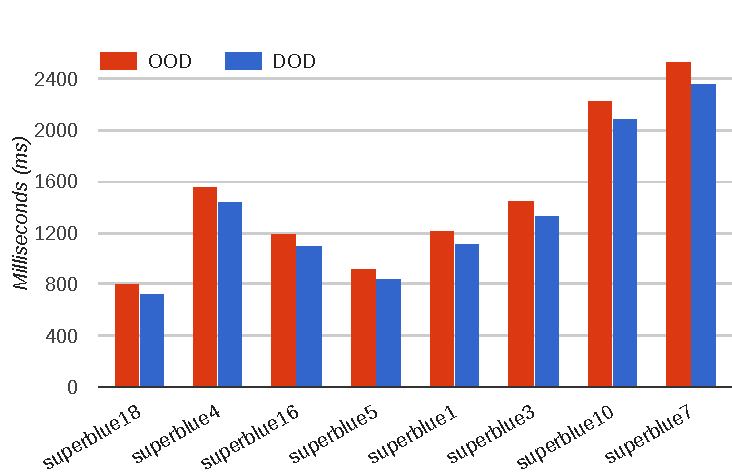
\includegraphics[width=0.7\linewidth]{img/results/runtimeProblemC_sequential_rtree}
    \caption[Tempo de execução Problema~C versão sequencial]{Tempo de execução para a implementação sequencial da Clusterização de Registradores}
    \label{fig:runtimeProblemC_sequential_rtree}
\end{figure}

\subsection{Execução Paralela}
\label{subsec:execucaoParalelaProblemaC}

Com objetivo de avaliar o comportamento das estruturas de dados em ambientes paralelos, foi implementado uma versão paralela do algoritmo K-Means.
A Figura~\ref{fig:missProblemC_parallel_rtree} apresenta o número total de cache misses (eixo Y) em milhões para cada circuito avaliado (eixo X) na implementação paralela.  
Pode-se notar que o número total de cache misses reduziu comparado as versões sequenciais. Isto se deve ao fato de que a implementação paralela usa os caches L1 e L2 de todos os núcleos, aumentando a quantidade de memória disponível. Outro benefício é que o terceiro nível da cache (L3) é compartilhado entre todos os cores do processador.
O número de falhas na cache para \ac{dod} (de $7M$ a $131M$) foi, em média, $20\%$ menor do que o alcançado pelo \ac{ood} (de $17M$ a $159M$). Este resultado demonstra que, como esperado, a organização de dados levou a um número menor de cache misses, mesmo para a implementação paralela.

\begin{figure}[ht]
    \centering
    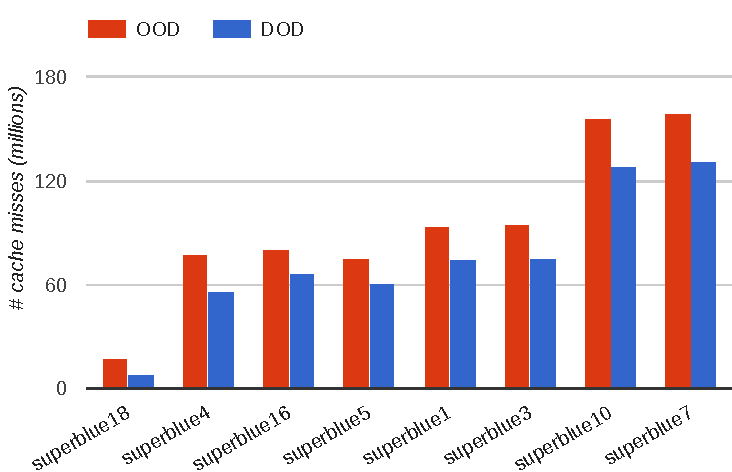
\includegraphics[width=0.7\linewidth]{img/results/missProblemC_parallel_rtree}
    \caption[Cache misses Problema~C versão paralela]{Número de cache misses para a implementação paralela de Clusterização de Registradores}
    \label{fig:missProblemC_parallel_rtree}
\end{figure}

A redução de cache misses impactou novamente no tempo de execução. A Figura~\ref{fig:runtimeProblemC_parallel_rtree} mostra os resultados de tempo de execução (eixo Y) em milissegundos para a implementação paralela. Os tempos de execução do \ac{dod} foram entre $264ms$ e $769ms$, enquanto que os tempos de execução da implementação que utilizou \ac{ood} foram entre $ 300ms $ e $ 896ms $. Portanto, o modelo de programação \ac{dod} é, em média, $ 15.5\% $ mais rápido que o modelo \ac{ood} quando ambos são paralelizados.


\begin{figure}[ht]
    \centering
    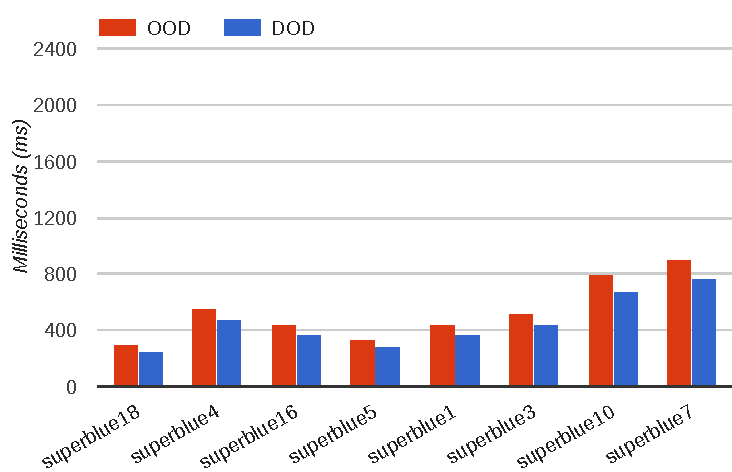
\includegraphics[width=0.7\linewidth]{img/results/runtimeProblemC_parallel_rtree}
    \caption[Tempo de execução Problema~C versão paralela]{Tempo de execução para a implementação paralela da Clusterização de Registradores}
    \label{fig:runtimeProblemC_parallel_rtree}
\end{figure}

Observe que, enquanto a implementação sequencial \ac{dod} é em média $ 7.5 \% $ mais rápida do que a implementação \ac{ood}, na implementação paralela essa diferença aumentam para $ 15 \% $.
Esses resultados mostram que a aceleração alcançada pela implementação paralela é maior quando aplicada usando o modelo de programação \ac{dod}, mesmo que a diferença no número de cache misses seja menor entre as implementações ($ 20 \% $ no cenário paralelo comparado a $ 24 \% $ no cenário sequencial).

Na verdade, considerando apenas as versões orientadas a dados (\ac{dod}), a implementação paralela alcançou um speedup\footnote{A métrica \textit{speedup} representa a relação entre os tempos de execução da solução sequencial e a solução paralela para um determinado número de threads.} médio de $ 3,04 $ em relação a implementação sequencial, enquanto ao comparar as duas versões  orientadas a objetos (\ac{ood}) speedup foi de apenas $ 2,78 $.
Um possível motivo para esses resultados pode advir de que o tempo de acesso à memória seja um fator mais relevante nas implementações paralelas do que nas sequenciais, tornando a programação com \ac{dod} ainda mais eficiente neste cenário.


\section{Síntese dos Resultados e Perspectivas}
\label{sec:sintese_resultado}

Nesta Seção será apresentados brevemente uma síntese dos resultados preliminares obtidos até a escrita deste documento. Posteriormente serão apresentadas as perspectivas de melhorias destes resultados.

A Tabela~\ref{tab:sintese_resultados} apresenta um breve resumo das reduções/acréscimos médios da técnica \ac{dod} sobre a técnica \ac{ood} no número de cache misses e tempo de execução.
Nesta tabela, números negativos em cache misses significam que a técnica \ac{dod} resultou em menor número de cache misses.
Ao passo que, números negativos no tempo de execução representam que a técnica \ac{dod} executou mais rápido que a técnica \ac{ood}. 

É possível identificar, tendo como base a Tabela~\ref{tab:sintese_resultados}, de que existem classes de problemas cujo o modelo de programação \ac{dod} pode superar em até dezesseis vezes ($16 \times$) o modelo de programação \ac{ood}. 
Porém, no caso em que o modelo \ac{dod} foi inferior no desempenho, a modularidade e a engenharia de software continuaram sendo superiores às que foram implementadas seguindo o modelo \ac{ood}.


\begin{table}[h]
\centering
\caption{Síntese dos resultados preliminares.}
\label{tab:sintese_resultados}
\resizebox{\textwidth}{!}{
\begin{tabular}{c|r|r|r|r|}
\cline{2-5}
                                 & \multicolumn{2}{c|}{Execução Sequencial}                                               & \multicolumn{2}{c|}{Execução Paralela}                                                 \\ \cline{2-5} 
                                 & \multicolumn{1}{c|}{\# Cache misses} & \multicolumn{1}{c|}{Tempo de Execução} & \multicolumn{1}{c|}{\# Cache misses} & \multicolumn{1}{c|}{Tempo de Execução} \\ \hline
\multicolumn{1}{|c|}{Problema A} & - 90\%                              & - 94\%                                & ---                                     & ---                                   \\ \hline
\multicolumn{1}{|c|}{Problema B} & + 10\%                              & + 6\%                                 &  ---                                    & ---                                   \\ \hline
\multicolumn{1}{|c|}{Problema C} & - 24\%                              & - 7.5\%                               & - 20\%                                  & - 15.5\%                              \\ \hline
\end{tabular}
}
\end{table}

Como perspectivas para melhorar ainda mais a organização dos dados, pretende-se implementar um modelo de \textit{entity-component system} que suporte a ordenação das propriedades de uma entidade.
Suportar a ordenação das propriedades possivelmente irá melhorar a performance das implementações.
Uma vez que, em determinadas tarefas é importante acessar os dados em uma ordem prevista.

Na Figura~\ref{fig:sorting_data_example}~(a) pode-se observar o mapeamento da estimativa de comprimento das interconexões, utilizando a técnica \ac{dod}, sem nenhum agrupamento nos dados.
Já na Figura~\ref{fig:sorting_data_example}~(b) é apresentado um possível agrupamento dos dados em relação a cada interconexão.
Este agrupamento reduziria o número de falhas na cache pois, para estimar o comprimento de uma interconexão, é necessário percorrer as posições dos pinos pertencentes a mesma interconexão.
Sendo estas posições armazenadas contiguamente, cada bloco recuperado pelo cache miss é melhor aproveitado.


\begin{figure}[ht]
    \centering
    \subfigure[Dados sem agrupamento]{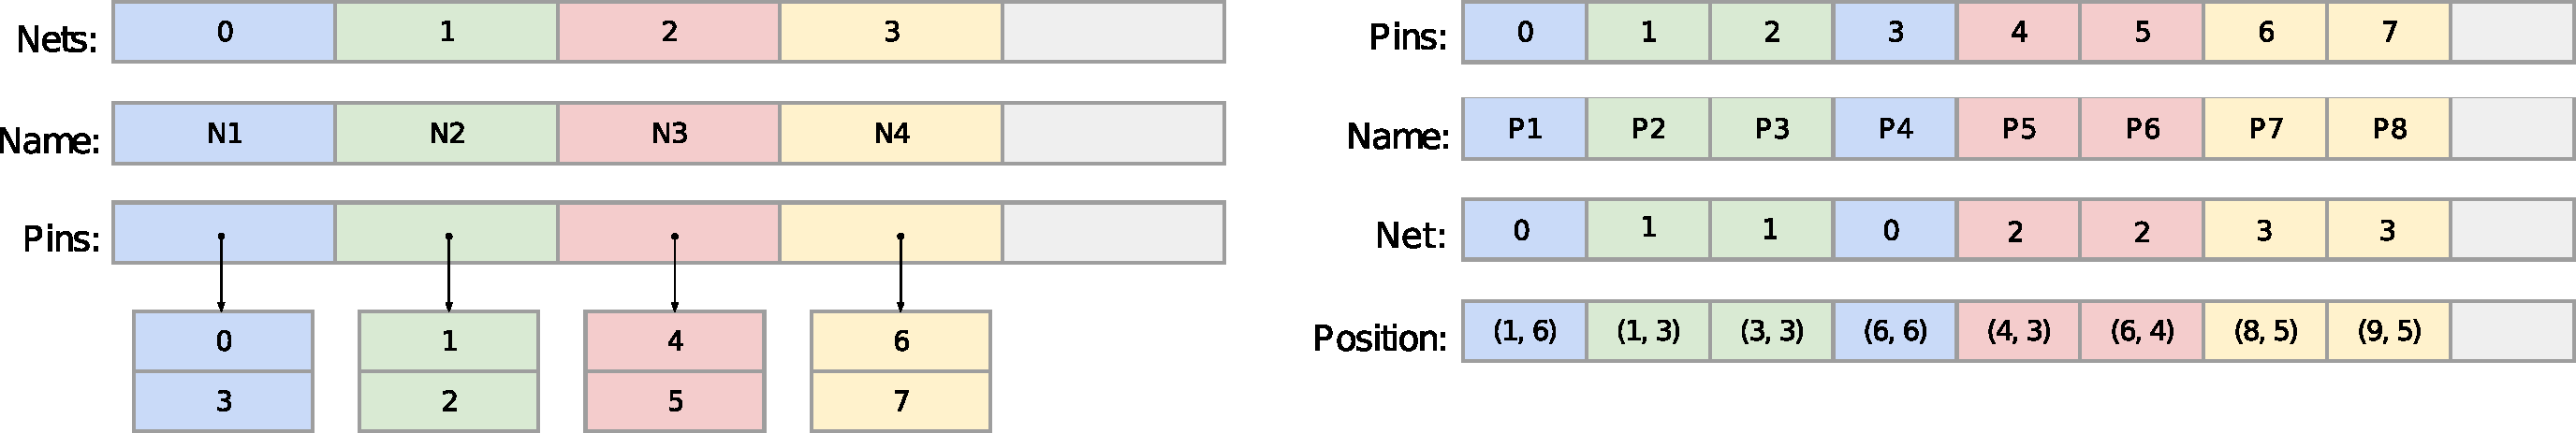
\includegraphics[width=\linewidth]{img/results/sorting_data_example_original}}
    
    \subfigure[Dados agrupados pelas interconexões]{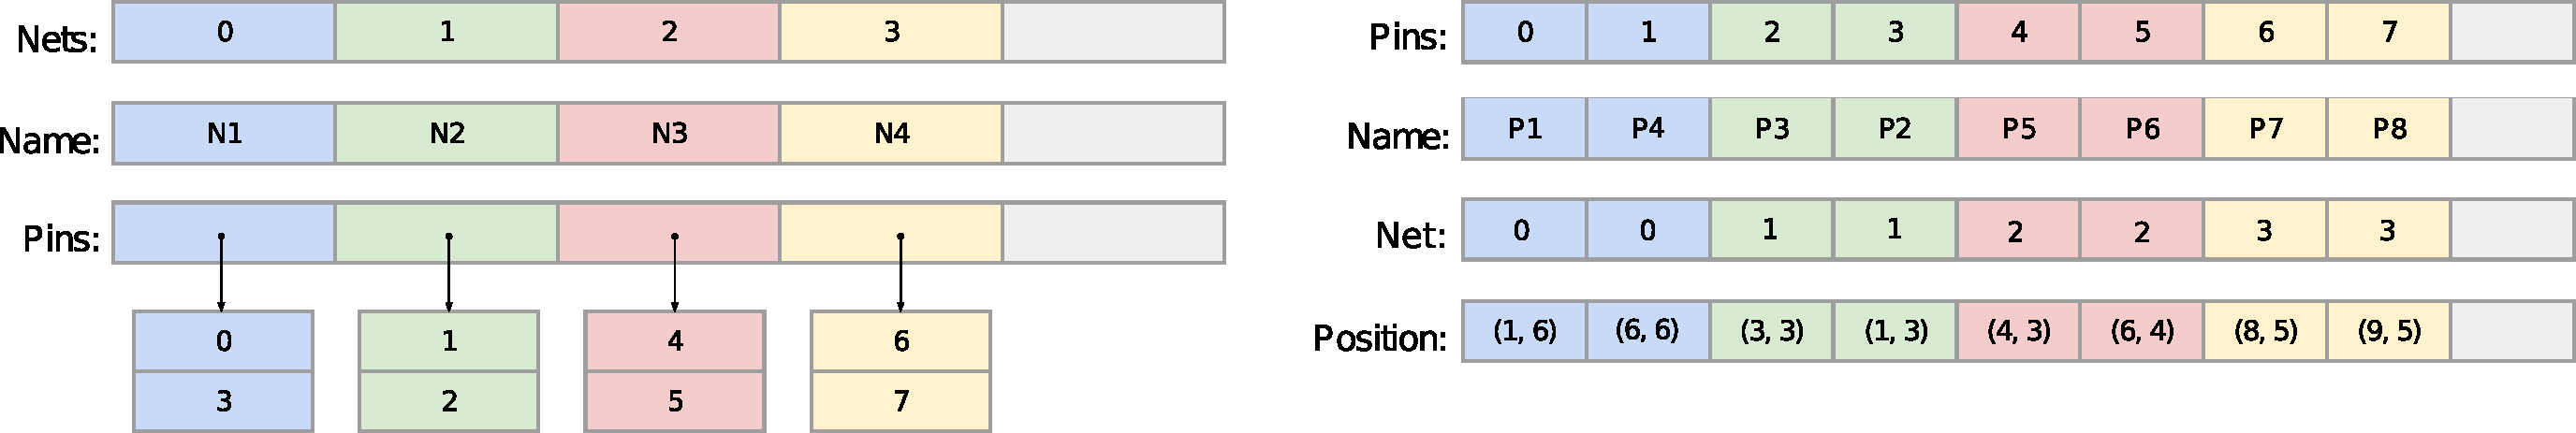
\includegraphics[width=\linewidth]{img/results/sorting_data_example_grouping}}
    \caption[Exemplo de agrupamento dos dados]{Exemplo de possível agrupamento nos dados para problema de estimativa do comprimento de interconexão. Cada propriedade está contiguamente armazenada em memória. (a) representa as propriedades sem nenhum agrupamento de dados. (b) representa os mesmos dados apresentados em (a) porém, com as interconexões propriedades agrupadas pelas interconexões.}
    \label{fig:sorting_data_example}
\end{figure}